\section{2020 年 11 月 24 日答疑记录}

本次答疑中的问题均为指数、对数相关问题, 知识点可参考 ``2020 年 11 月 21 日答疑记录'' 第二部分.

\subsection{对数函数的单调性和定义域}

\begin{example}\label{exa:201209-1910}
    已知 $0<a<1$, $\log_a m< \log_a n< 0$, 比较 $m$, $n$ 与 $1$ 的大小.
\end{example}
\begin{solution}
    由 $0=\log_a 1$ 知不等式化为 $\log_a m< \log_a n< \log_a 1$. 因为 $0<a<1$, 所以对数函数 $f(x)= \log_a x$ 在 $(0,+\infty)$ 上单调递减, 则 $m>n>1$.
\end{solution}
\begin{remark}
    若例~\ref{exa:201209-1910} 中的不等式 ``$\log_a m< \log_a n< 0$'' 改为 ``$\log_a m> \log_a n> 0$'', 则答案建议写为: $0<m<n<1$ (即对数函数中的真数一定为正数).
\end{remark}

\begin{example}
    (1) 已知 $a$, $b\in\realnum$, 则 ``$a<b$'' 是 ``$\log_2 a<\log_2 b$'' 的什么条件?
    
    (2) 已知 $x\in\realnum$, 则 ``$x<0$'' 是 ``$\ln(x+1)<0$'' 的什么条件?
\end{example}
\begin{solution}
    (1) 由例~\ref{exa:201209-1910} 的解答及注可知, $\log_2 a<\log_2 b$ 等价于 $0<a<b$, 所以 ``$a<b$'' 是 ``$\log_2 a<\log_2 b$'' 的必要不充分条件.
    
    (2) $\ln(x+1)<0$ 等价于 $0<x+1<1$ 即 $-1<x<0$, 所以 ``$x<0$'' 也是 ``$\ln(x+1)<0$'' 的必要不充分条件
\end{solution}

\begin{example}
    已知 $a>0$ 且 $a\neq 1$, 画出函数 $f(x)= \log_a x$, $g(x)=a^x$, $h(x)= x+a$ 在同一坐标系内图形的各种可能情形.
\end{example}
\begin{solution}
    对数函数和指数函数的单调性均由底数 (本例中的 $a$) 与 $1$ 的大小决定, 所以只需分 $0<a<1$ 与 $a>1$ 来讨论. 具体绘图如下:
    
    \begin{center}
        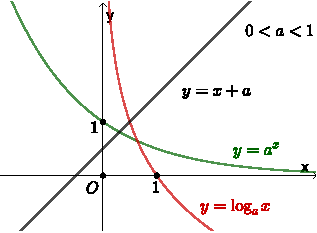
\includegraphics[scale=1]{2020-1209-2000-crop}\qquad
        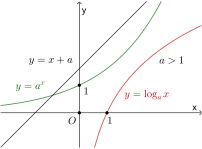
\includegraphics[scale=1]{2020-1209-2010-crop}
    \end{center}
\end{solution}

\subsection{比较多个数的大小}

关于比较多个数的大小的一般方法, 可参考 ``2020 年 11 月 21 日答疑记录'' 末尾的说明.

\begin{example}
    比大小: (1) $a=0.4^2$, $b=3^{0.4}$, $c=\log_4 0.3$;
    
    (2) $a=2^{1.2}$, $b=\biggl(\dfrac12\biggr)^{-0.8}$, $c=2\log_4 2$;
    
    (3) $a=\log_3 \mathrm{e}$, $b=\ln 3$, $c=\log_3 2$.
\end{example}
\begin{solution}
    (1) 分别考查函数 $f(x)=0.4^x$, $g(x)=3^x$, $h(x)=\log_4 x$ 的图形可知, $a=f(2)\in(0,1)$ (实际上 $a=0.16$), $b=g(0.4)\in(1,3)$, $c=h(0.3)\in(-\infty,0)$, 所以 $c<a<b$.
    
    (2) 分别考查函数 $f(x)=2^x$, $g(x)= \log_5 x$ 的图形可知, $a=f(1.2)\in(2,4)$, $b=2^{0.8}=f(0.8)\in(1,2)$, $c=\log_5 4=g(4)\in(0,1)$, 所以 $c<b<a$.
    
    (3) 分别考查函数 $f(x)=\log_3 x$, $g(x)=\ln x$ 的图形可知, $a=f(\mathrm{e})\in(0,1)$ (注意 $\mathrm{e}=2.718\cdots$), $b=g(3)\in(1,2)$ ($\ln x$ 的底数是 $\mathrm{e}$), $c=f(2)\in(0,1)$, 而 $f(2)<f(\mathrm{e})$, 所以 $c<a<b$.
\end{solution}



